\chapter{Theoretical framework}

This chapter lays out the theoretical foundations used throughout the thesis and is divided into four main sections. The first section (\secref{sec:nanophotonics}) covers the fundamental physics governing nanophotonic problems in the single-physics picture. The second section (\secref{sec:fem}) provides background on solving nanophotonic problems numerically using the finite element method. The third section (\secref{sec:coupled}) presents the concept of coupled nanophotonic systems in the multiphysics picture. Finally, the fourth section (\secref{sec:topopt_theory}) presents a framework for the topology optimization of multiphysics systems.

%\begin{figure}[tb]
%    \centering
%    \makebox[\textwidth][c]{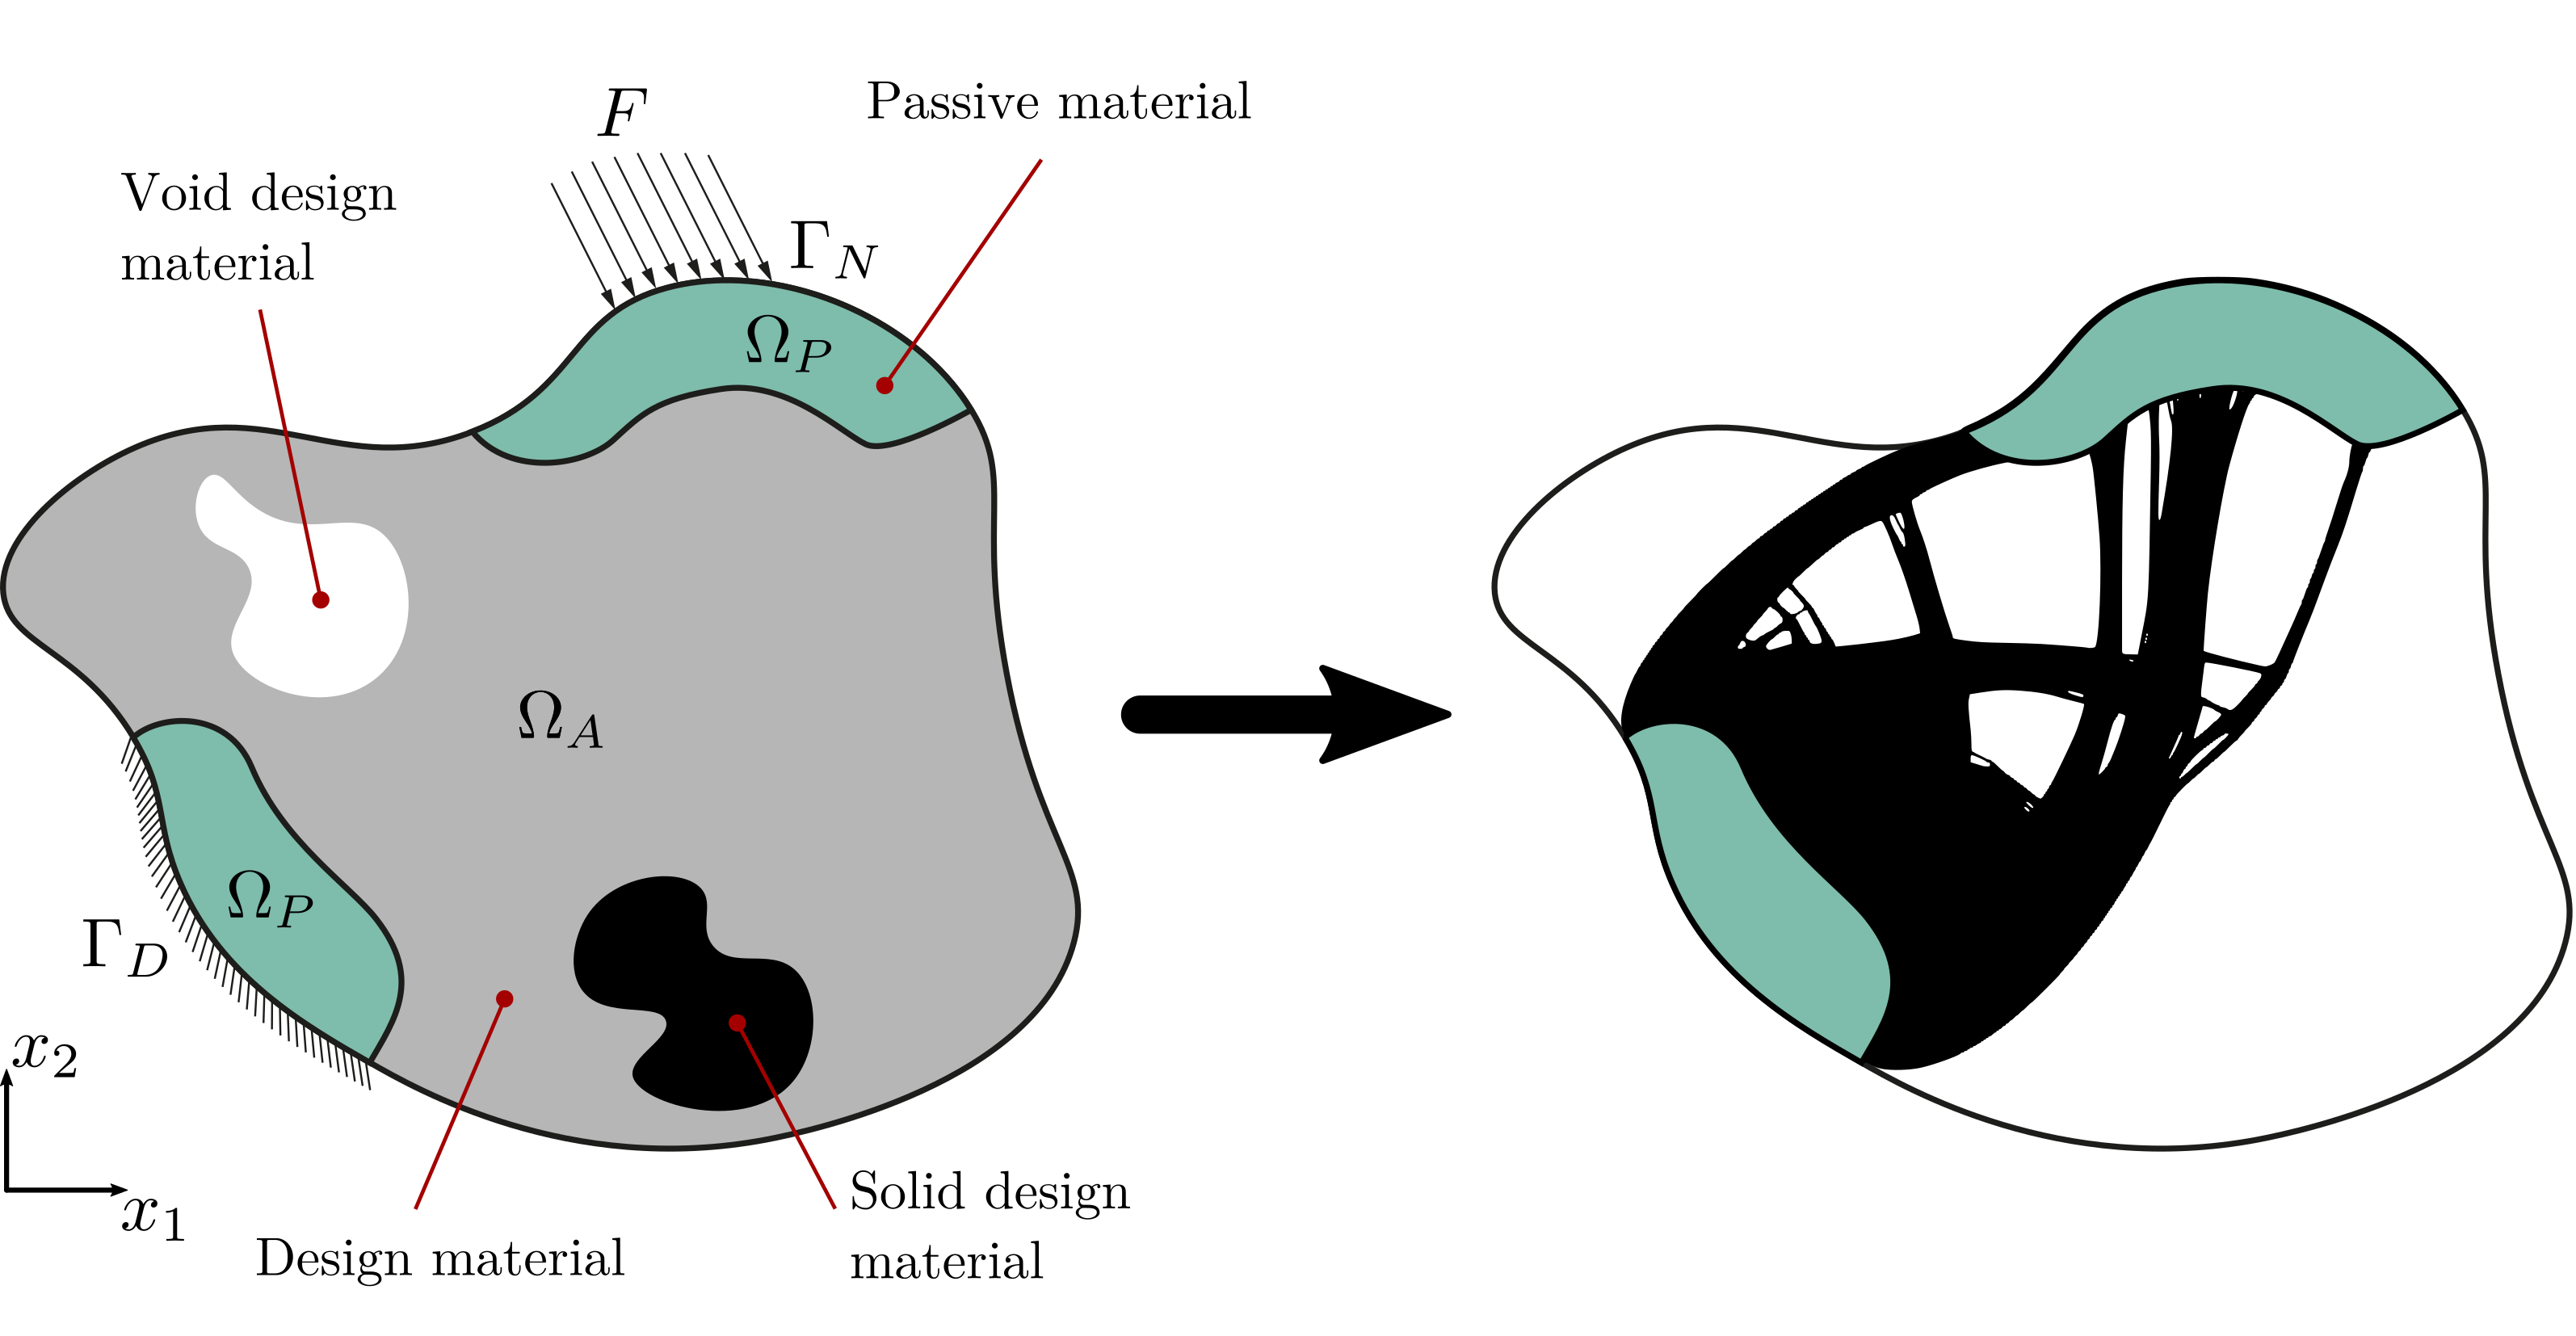
\includegraphics[width=1\imwidth]{figures/simpModel.png}}%
%    \caption{Bla bla bla...}
%    \label{fig:illustateTopOpt}
%\end{figure}

%\begin{equation}
%    (EIu'')'' = q
%\end{equation}

%\begin{figure}[tb]
%    \centering
%    \makebox[\textwidth][c]{\begin{tikzpicture}[remember picture]
    \begin{scope}[xshift=0mm]
        % angle (deg)
        \newcommand\ai{10}
        % line width
        \newcommand\wi{1pt}
        % cell size
        \newcommand\cellsize{3}
        % Rank-$N$ size
        \newcommand\di{0.75}

        % cell
        \draw[gray!10,   fill=gray!10, rotate around={\ai:(0,0)}] (0,0) rectangle (\cellsize,\cellsize) node (rect1) {};
        \draw[black!60, fill=black!60, rotate around={\ai:(0,0)}] (0,0) rectangle (\di,\cellsize);

        % orientation frame
        \draw[black, -stealth, line width=\wi, rotate around={\ai:({\di*cos(\ai) - \cellsize/2*sin(\ai)},{\di*sin(\ai) + \cellsize/2*cos(\ai)})}] ({\di*cos(\ai) - \cellsize/2*sin(\ai)},{\di*sin(\ai) + \cellsize/2*cos(\ai)}) -- ({\di*cos(\ai) - \cellsize/2*sin(\ai) + 0.75},{\di*sin(\ai) + \cellsize/2*cos(\ai)});
        \draw[black, -stealth, line width=\wi, rotate around={\ai:({\di*cos(\ai) - \cellsize/2*sin(\ai)},{\di*sin(\ai) + \cellsize/2*cos(\ai)})}] ({\di*cos(\ai) - \cellsize/2*sin(\ai)},{\di*sin(\ai) + \cellsize/2*cos(\ai)}) -- ({\di*cos(\ai) - \cellsize/2*sin(\ai)},{\di*sin(\ai) + \cellsize/2*cos(\ai) + 0.75});

        % local frame
        \draw[black, -stealth, dashed, line width=\wi] (0,0) -- ({\cellsize + 0.8},0);
        \draw[black, -stealth, dashed, line width=\wi] (0,0) -- (0,{\cellsize + 0.8});

        % ruler
        \draw[black, |-|, line width=\wi, rotate around={\ai:(0,0)}] (0,0) -- (\cellsize,0);
        \draw[black,  -|, line width=\wi, rotate around={\ai:(0,0)}] (0,0) -- (\di,0);

        % arc
        \draw[black, dotted, line width=\wi] (\cellsize,0) arc (0:\ai:\cellsize);

        % annotation
        \draw (\cellsize + 0.7, -0.3) node {$x_1 / \epsilon^3$};
        \draw (-0.5, \cellsize + 0.8) node {$x_2 / \epsilon^3$};
        \draw (\cellsize/2,-0.75) node {Rank-$1$};

        \draw[rotate around={{\ai/2}:(0,0)}] ({\cellsize+0.3},0) node {$\theta_1$};

        \draw[rotate around={{\ai}:(0,0)}] ({\di/2},0.4) node [rotate around={{\ai}:(0,0)}] {$\mu_1$};
        \draw[rotate around={{\ai}:(0,0)}] ({(\cellsize - \di)/2 + \di},0.4) node [rotate around={{\ai}:(0,0)}] {$1-\mu_1$};

        \draw[rotate around={{\ai}:(0,0)}] ({0+0.4},{\cellsize-0.4}) node [rotate around={{\ai}:(0,0)}] {$(+)$};
        \draw[rotate around={{\ai}:(0,0)}] ({\cellsize-0.4},{\cellsize-0.4}) node [rotate around={{\ai}:(0,0)}] {$(-)$};
        \coordinate (A) at (rect1.north);


        \draw[rotate around={\ai:({\di*cos(\ai) - \cellsize/2*sin(\ai)},{\di*sin(\ai) + \cellsize/2*cos(\ai)})}] ({\di*cos(\ai) - \cellsize/2*sin(\ai)+1} , {\di*sin(\ai) + \cellsize/2*cos(\ai) + 0.2}) node {$\mathbf{n}_1$};
        \draw[rotate around={\ai:({\di*cos(\ai) - \cellsize/2*sin(\ai)},{\di*sin(\ai) + \cellsize/2*cos(\ai)})}] ({\di*cos(\ai) - \cellsize/2*sin(\ai) + 0.3} , {\di*sin(\ai) + \cellsize/2*cos(\ai) + 1}) node {$\mathbf{m}_1$};



    \end{scope}
    \begin{scope}[xshift=45mm]
        % angle (deg)
        \newcommand\ai{15}
        % line width
        \newcommand\wi{1pt}
        % cell size
        \newcommand\cellsize{3}
        % Rank-$N$ size
        \newcommand\di{0.6}

        % cell
        \draw[gray!40,   fill=gray!40, rotate around={\ai:(0,0)}] (0,0) rectangle (\cellsize,\cellsize) node (rect2) {};
        \draw[black!60, fill=black!60, rotate around={\ai:(0,0)}] (0,0) rectangle (\di,\cellsize);

        % orientation frame
        \draw[black, -stealth, line width=\wi, rotate around={\ai:({\di*cos(\ai) - \cellsize/2*sin(\ai)},{\di*sin(\ai) + \cellsize/2*cos(\ai)})}] ({\di*cos(\ai) - \cellsize/2*sin(\ai)},{\di*sin(\ai) + \cellsize/2*cos(\ai)}) -- ({\di*cos(\ai) - \cellsize/2*sin(\ai) + 0.75},{\di*sin(\ai) + \cellsize/2*cos(\ai)});
        \draw[black, -stealth, line width=\wi, rotate around={\ai:({\di*cos(\ai) - \cellsize/2*sin(\ai)},{\di*sin(\ai) + \cellsize/2*cos(\ai)})}] ({\di*cos(\ai) - \cellsize/2*sin(\ai)},{\di*sin(\ai) + \cellsize/2*cos(\ai)}) -- ({\di*cos(\ai) - \cellsize/2*sin(\ai)},{\di*sin(\ai) + \cellsize/2*cos(\ai) + 0.75});

        % local frame
        \draw[black, -stealth, dashed, line width=\wi] (0,0) -- ({\cellsize + 0.8},0);
        \draw[black, -stealth, dashed, line width=\wi] (0,0) -- (0,{\cellsize + 0.8});

        % ruler
        \draw[black, |-|, line width=\wi, rotate around={\ai:(0,0)}] (0,0) -- (\cellsize,0);
        \draw[black,  -|, line width=\wi, rotate around={\ai:(0,0)}] (0,0) -- (\di,0);

        % arc
        \draw[black, dotted, line width=\wi] (\cellsize,0) arc (0:\ai:\cellsize);

        % annotation
        \draw (\cellsize + 0.7, -0.3) node {$x_1 / \epsilon^2$};
        \draw (-0.5, \cellsize + 0.8) node {$x_2 / \epsilon^2$};
        \draw (\cellsize/2,-0.75) node {Rank-$2$};

        \draw[rotate around={{\ai/2}:(0,0)}] ({\cellsize+0.3},0) node {$\theta_2 + \pi/4$};

        \draw[rotate around={{\ai}:(0,0)}] ({\di/2},0.4) node [rotate around={{\ai}:(0,0)}] {$\mu_2$};
        \draw[rotate around={{\ai}:(0,0)}] ({(\cellsize - \di)/2 + \di},0.4) node [rotate around={{\ai}:(0,0)}] {$1-\mu_2$};

        \draw[rotate around={{\ai}:(0,0)}] ({0+0.4},{\cellsize-0.4}) node [rotate around={{\ai}:(0,0)}] {$(+)$};
        \draw[rotate around={{\ai}:(0,0)}] ({\cellsize-0.9},{\cellsize-0.4}) node [rotate around={{\ai}:(0,0)}] (B) {$(\text{Rank-1})$};
        \coordinate (B2) at (rect2.north);


        \draw[rotate around={\ai:({\di*cos(\ai) - \cellsize/2*sin(\ai)},{\di*sin(\ai) + \cellsize/2*cos(\ai)})}] ({\di*cos(\ai) - \cellsize/2*sin(\ai)+1} , {\di*sin(\ai) + \cellsize/2*cos(\ai) + 0.2}) node {$\mathbf{n}_2$};
        \draw[rotate around={\ai:({\di*cos(\ai) - \cellsize/2*sin(\ai)},{\di*sin(\ai) + \cellsize/2*cos(\ai)})}] ({\di*cos(\ai) - \cellsize/2*sin(\ai) + 0.3} , {\di*sin(\ai) + \cellsize/2*cos(\ai) + 1}) node {$\mathbf{m}_2$};


    \end{scope}
    \begin{scope}[xshift=90mm]
        % angle (deg)
        \newcommand\ai{20}
        % line width
        \newcommand\wi{1pt}
        % cell size
        \newcommand\cellsize{3}
        % Rank-$N$ size
        \newcommand\di{1.0}

        % cell
        \draw[gray!60,   fill=gray!60, rotate around={\ai:(0,0)}] (0,0) rectangle (\cellsize,\cellsize);
        \draw[black!60, fill=black!60, rotate around={\ai:(0,0)}] (0,0) rectangle (\di,\cellsize);

        % orientation frame
        \draw[black, -stealth, line width=\wi, rotate around={\ai:({\di*cos(\ai) - \cellsize/2*sin(\ai)},{\di*sin(\ai) + \cellsize/2*cos(\ai)})}] ({\di*cos(\ai) - \cellsize/2*sin(\ai)},{\di*sin(\ai) + \cellsize/2*cos(\ai)}) -- ({\di*cos(\ai) - \cellsize/2*sin(\ai) + 0.75},{\di*sin(\ai) + \cellsize/2*cos(\ai)});
        \draw[black, -stealth, line width=\wi, rotate around={\ai:({\di*cos(\ai) - \cellsize/2*sin(\ai)},{\di*sin(\ai) + \cellsize/2*cos(\ai)})}] ({\di*cos(\ai) - \cellsize/2*sin(\ai)},{\di*sin(\ai) + \cellsize/2*cos(\ai)}) -- ({\di*cos(\ai) - \cellsize/2*sin(\ai)},{\di*sin(\ai) + \cellsize/2*cos(\ai) + 0.75});

        % local frame
        \draw[black, -stealth, dashed, line width=\wi] (0,0) -- ({\cellsize + 0.8},0);
        \draw[black, -stealth, dashed, line width=\wi] (0,0) -- (0,{\cellsize + 0.8});

        % ruler
        \draw[black, |-|, line width=\wi, rotate around={\ai:(0,0)}] (0,0) -- (\cellsize,0);
        \draw[black,  -|, line width=\wi, rotate around={\ai:(0,0)}] (0,0) -- (\di,0);

        % arc
        \draw[black, dotted, line width=\wi] (\cellsize,0) arc (0:\ai:\cellsize);

        % annotation
        \draw (\cellsize + 0.7, -0.3) node {$x_1 / \epsilon$};
        \draw (-0.5, \cellsize + 0.8) node {$x_2 / \epsilon$};
        \draw (\cellsize/2,-0.75) node {Rank-$3$};

        \draw[rotate around={{\ai/2}:(0,0)}] ({\cellsize+0.3},0) node {$\theta_3 - \pi/2$};

        \draw[rotate around={{\ai}:(0,0)}] ({\di/2},0.4) node [rotate around={{\ai}:(0,0)}] {$\mu_3$};
        \draw[rotate around={{\ai}:(0,0)}] ({(\cellsize - \di)/2 + \di},0.4) node [rotate around={{\ai}:(0,0)}] {$1-\mu_3$};

        \draw[rotate around={{\ai}:(0,0)}] ({0+0.4},{\cellsize-0.4}) node [rotate around={{\ai}:(0,0)}] {$(+)$};
        \draw[rotate around={{\ai}:(0,0)}] ({\cellsize-0.9},{\cellsize-0.4}) node [rotate around={{\ai}:(0,0)}] (C) {$(\text{Rank-2})$};


        \draw[rotate around={\ai:({\di*cos(\ai) - \cellsize/2*sin(\ai)},{\di*sin(\ai) + \cellsize/2*cos(\ai)})}] ({\di*cos(\ai) - \cellsize/2*sin(\ai)+1} , {\di*sin(\ai) + \cellsize/2*cos(\ai) + 0.2}) node {$\mathbf{n}_3$};
        \draw[rotate around={\ai:({\di*cos(\ai) - \cellsize/2*sin(\ai)},{\di*sin(\ai) + \cellsize/2*cos(\ai)})}] ({\di*cos(\ai) - \cellsize/2*sin(\ai) + 0.3} , {\di*sin(\ai) + \cellsize/2*cos(\ai) + 1}) node {$\mathbf{m}_3$};

    \end{scope}
    \path[-latex,black,thick] (A) edge [bend left=50] (B);
    \path[-latex,black,thick] (B2) edge [bend left=50] (C);
\end{tikzpicture}}%
%    \caption{Bla bla bla...}
%    \label{fig:Rank}
%\end{figure}

\section{Nanophotonics -- light as an electromagnetic
  wave}\label{sec:nanophotonics}

  In classical optics, light is treated as an electromagnetic wave, and can be described mathematically 
  using different physical models. As shown in \figref{fig:EM_regime},
  when the characteristic sizes ($s$) of objects are very different from the electromagnetic wave's
  wavelength ($\lambda$),
  regime-specific models can be used to describe optical phenomena:
  \begin{itemize}
      \item \textbf{Geometrical or ray optics ($s \gg \lambda$):} When objects
   are much larger than the wavelength, light can be modeled as straight-line rays,
   which might refract or reflect in the presence of different media, such as
   lenses and mirrors.
      \item \textbf{Quasistatics and lumped circuit models ($s \ll \lambda$):}
   When objects are much smaller than the wavelength, the electromagnetic fields vary slowly over the object's dimensions 
   and can be approximated quasistatically. For instance, electronic devices
   can be modeled in this regime using circuit models with sources ($V$) and lumped elements, 
   like resistors ($R$), capacitors ($C$) and coils ($L$).
  \end{itemize}

  In the fields of nano-optics and nanophotonics, the visible
  (\(\lambda \approx 400\)--\(800\) nm) and near-infrared (\(\lambda \approx 800\)--\(2500\)
  nm)
  spectral regions are most commonly explored, and components often have nano- to
  microscale dimensions. As a result, the \textbf{wave-optics} regime ($s
      \sim \lambda$) needs to be considered,
  where it is generally not possible to resort to simpler models like ray optics or
  quasistatic and lumped circuits models,
  and instead one needs to solve Maxwell's equations. Given the complexity of
  Maxwell's
  equations, very few problems (e.g., problems with high symmetry, separability,
  few parameters)
  can be solved analytically, and most problems require
  numerical solutions [e.g., obtained via the finite element method (\secref{sec:fem})].

\subsection*{The macroscopic Maxwell's equations}

Light propagation in macroscopic electromagnetic systems can be
described by the \emph{macroscopic} Maxwell's equations. The \textbf{time-domain Maxwell's
equations} in a linear, isotropic, and homogeneous medium are~\cite{maxwell1873,novotny}
\begin{align}
    \nabla \times \bm{\mathcal{E}} (\mathbf{r},t)            & = - \frac{\partial
    \bm{\mathcal{B}}(\mathbf{r},t)}{\partial t}, \quad \quad & \text{(Faraday's
    law)} \label{eq:faraday}                                                                                         \\
    \nabla \times \bm{\mathcal{H}} (\mathbf{r},t)            & = \frac{\partial
        \bm{\mathcal{D}}(\mathbf{r},t)}{\partial t} + \bm{\mathcal{J}}(\mathbf{r},t),
    \quad \quad                                              & \text{(Ampère's law)} \label{eq:ampere}               \\
    \nabla \cdot \bm{\mathcal{D}} (\mathbf{r},t)             & =
    \varrho_q(\mathbf{r},t), \quad \quad                & \text{(Gauss's law for electricity)}
    \label{eq:gauss_E}                                                                                               \\
    \nabla \cdot \bm{\mathcal{B}} (\mathbf{r},t)             & = 0, \quad \quad
                                                             & \text{(Gauss's law for magnetism)} \label{eq:Gauss_B}
\end{align}
where $\mathbf{r}$ is the position vector, $t$ is time, $\bm{\mathcal{E}}$ and $\bm{\mathcal{H}}$ are the time-dependent electric
and magnetic (induction) fields, respectively,
$\bm{\mathcal{D}}$ is the time-dependent electric displacement field,
$\bm{\mathcal{B}}$ is the time-dependent magnetic (flux-density) field,
$\bm{\mathcal{J}}$ is the current density,
and $\varrho_q$ is the time-dependent charge density. % Maxwell's equations
%combine previously established
%physical laws, in 4 equations:
%\begin{itemize}
%    \item \textbf{Faraday's law} [\eqref{eq:faraday}] describes how a
%          time-varying magnetic field induces an electric field.
%    \item \textbf{Ampère's law} [\eqref{eq:ampere}] describes how a
%         time-varying electric field and electric current density induce a magnetic
%          field.
%    \item \textbf{Gauss's law for electricity} [\eqref{eq:gauss_E}]
%          describes how electric charges create an electric field.
%    \item \textbf{Gauss's law for magnetism} [\eqref{eq:Gauss_B}] states
%          that there are no magnetic monopoles, and thus the magnetic field lines are
%          closed loops.
%\end{itemize}
Note that the macroscopic fields in Maxwell's equations
are spatial averages of the
microscopic fields, and the charge and current densities are continuous in space
and time.
For an atomic-scale description of the electromagnetic fields, one can use the
\emph{microscopic}
Maxwell's equations, which include a quantized description of matter based on
discrete charged particles
(e.g., electrons, protons, etc.) and currents.

\begin{figure}[tb]
   \centering

   \makebox[\textwidth][c]{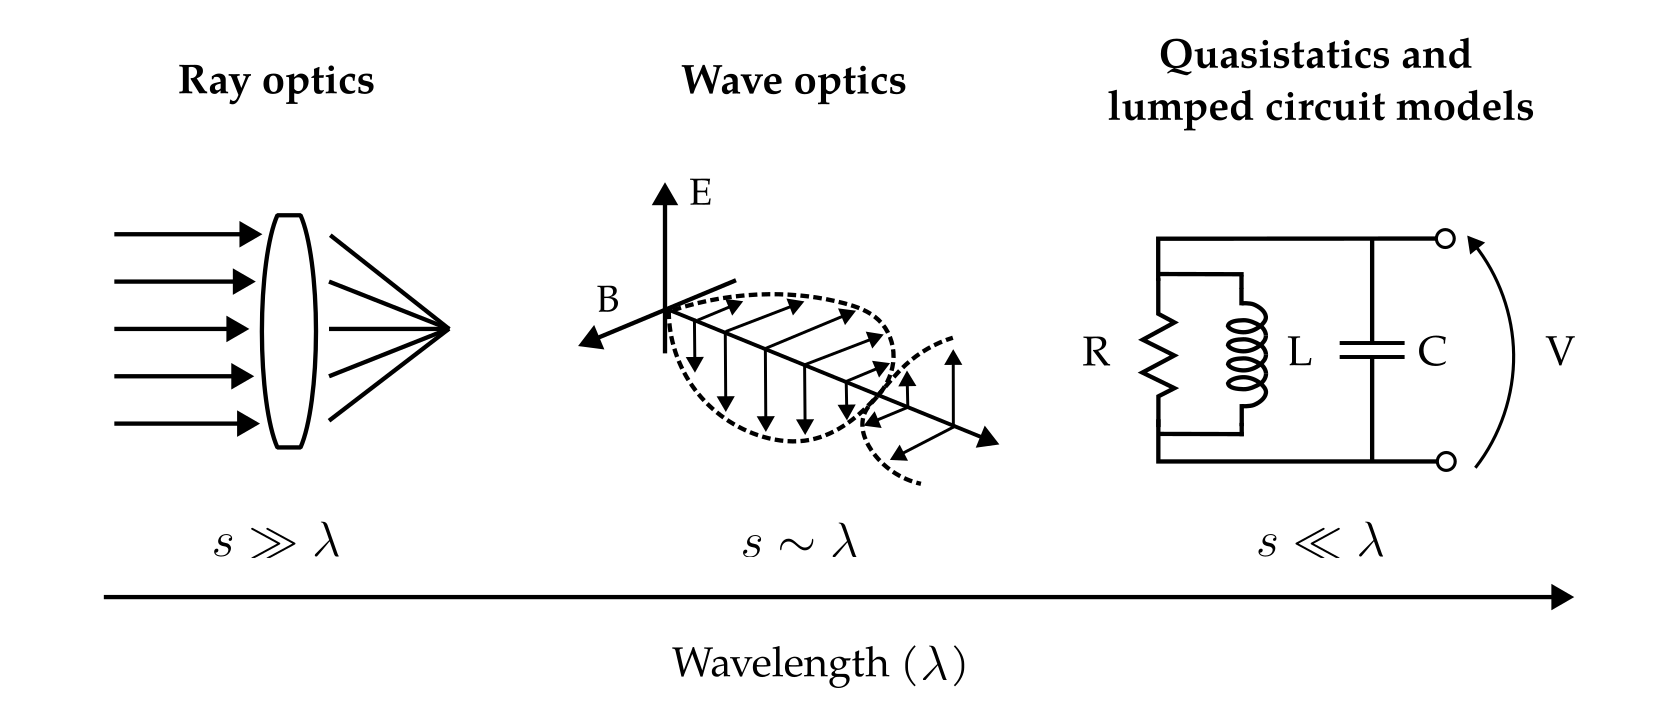
\includegraphics{figures/EM_regimes.png}}%%
   \caption{Different modeling regimes in electromagnetics based on the
       relation between the characteristic size of the objects ($s$) and the
       wavelength of light ($\lambda$). In wave optics, $E$ and $B$ refer to
       the electric and magnetic fields, respectively.}
   \label{fig:EM_regime}
\end{figure}

\subsection*{Material responses via the constitutive equations}

To understand how materials respond to electromagnetic fields, it is necessary to introduce the \textbf{constitutive equations}.
 For non-dispersive media, materials can be
modeled
with the presence of a time-dependent polarization $\bm{\mathcal{P}}$ and
magnetization $\bm{\mathcal{M}}$,
which relate the fields $\bm{\mathcal{D}}$ and $\bm{\mathcal{B}}$ to the fields
$\bm{\mathcal{E}}$ and
$\bm{\mathcal{H}}$ via the constitutive equations~\cite{novotny}
\begin{align}
    \bm{\mathcal{D}}(\mathbf{r}, t) & = \varepsilon(\mathbf{r}) \bm{\mathcal{E}}(\mathbf{r}, t) =
    \varepsilon_0 \bm{\mathcal{E}}(\mathbf{r}, t) + \bm{\mathcal{P}}(\mathbf{r}, t),
    \label{eq:D}                                                                \\
    \bm{\mathcal{B}}(\mathbf{r}, t) & =  \mu(\mathbf{r}) \bm{\mathcal{H}}(\mathbf{r},
    t) = \mu_0 \left[ \bm{\mathcal{M}}(\mathbf{r},
    t) + \bm{\mathcal{H}}(\mathbf{r}, t)\right] \label{eq:H},
\end{align}
where $\varepsilon_0$ is the free-space permittivity, $\mu_0$ is the free-space
permeability, $\varepsilon$ is the material permittivity, and 
$\mu$ is the material permeability. It is common to describe a medium
using the relative permittivity $\varepsilon_r=\varepsilon/\varepsilon_0$, which can be related to the material's refractive index~\cite{wooten}
\begin{equation}\label{eq:perm}
    \varepsilon_r = \varepsilon_r^\prime +
i \varepsilon_r^{\prime\prime} = \underbar{n}^2 = (n+ i\kappa)^2\,,
\end{equation}
where $\varepsilon_r^\prime$ is the real part of the relative permittivity, $i$ is the imaginary unit, $\varepsilon_r^{\prime\prime}$ is the imaginary part of the relative permittivity, $\underbar{n}$ is the complex refractive index, 
$n$ is the real refractive index and $\kappa$ is the extinction coefficient. 
The refractive index is a measure of how fast light propagates in a medium: $n=c/v$, where $v$ is the phase velocity of light in the medium, and 
$c=(\varepsilon_0 \mu_0)^{-1/2}$ is the speed of light in vacuum; while the extinction
coefficient ($\kappa$) and the imaginary part of the relative permittivity ($\varepsilon_r^{\prime\prime}=2n\kappa$) are related to the absorption of light in the medium.

The polarization and magnetization introduced in~\eqref{eq:D} and~\eqref{eq:H} also depend on the electromagnetic
fields. For instance, the
polarization can be written as a series expansion in powers of the electric
field
\begin{equation}\label{eq:polarization}
\bm{\mathcal{P}}=\mathcal{\varepsilon}_0 \bm{\mathcal{\chi}}^{(1)}
 \bm{\mathcal{E}}+\mathcal{\varepsilon}_0 \bm{\mathcal{\chi}}^{(2)}
 \bm{\mathcal{E}} \bm{\mathcal{E}}+\mathcal{\varepsilon}_0
 \bm{\mathcal{\chi}}^{(3)} \bm{\mathcal{E}} \bm{\mathcal{E}}
 \bm{\mathcal{E}}+\cdots,
\end{equation}
where $\bm{\mathcal{\chi}}^{(j)}$ is the $j^\text{th}$ order component of the
electric susceptibility. Note that in this thesis
we only consider linear materials\footnote{In some cases, we approximate nonlinearities perturbatively to linear
order (\secref{sec:laser})~\cite{ownpub4}.}, where only the first-order terms in the expansion are
considered. \\

\subsection*{Wave equations for electromagnetic fields}

Using Maxwell's equations and applying the curl operator to Faraday's law
    (\eqref{eq:faraday}) and Ampère's law (\eqref{eq:ampere}),
together with the constitutive relations (\eqref{eq:D} and
        \eqref{eq:H}), yields two
\textbf{wave equation}s for the electric and magnetic fields
\begin{equation}
    \begin{aligned}
         & \nabla \times \nabla \times \bm{\mathcal{E}}+\frac{1}{c^2}
        \frac{\partial^2 \bm{\mathcal{E}}}{\partial t^2}=-\mu_0
        \frac{\partial}{\partial t}\left(\bm{\mathcal{J}}+\frac{\partial
        \bm{\mathcal{P}}}{\partial t}+\nabla \times \bm{\mathcal{M}}\right), \\
         & \nabla \times \nabla \times \bm{\mathcal{H}}+\frac{1}{c^2}
        \frac{\partial^2 \bm{\mathcal{H}}}{\partial t^2}=\nabla \times
        \bm{\mathcal{J}}+\nabla \times \frac{\partial \bm{\mathcal{P}}}{\partial
            t}-\frac{1}{c^2} \frac{\partial^2 \bm{\mathcal{M}}}{\partial t^2}\,.
    \end{aligned}
\end{equation}
These
equations encapsulate the wave-like behavior of electromagnetic fields and
hold for arbitrary material properties.

\subsection*{Electromagnetics in the frequency domain}

The time dependence in Maxwell's equations can be separated by assuming
time-harmonic fields
\begin{equation}
 \bm{\mathcal{E}}(\mathbf{r}, t) = \Re \{ \mathbf{E}(\mathbf{r}) e^{-i\omega
 t} \}= \frac{1}{2}\left[ \mathbf{E}(\mathbf{r}) e^{-i\omega t} +
 \mathbf{E}^*(\mathbf{r}) e^{i\omega t}\right],
\end{equation}
where $\mathbf{E}$ is the complex electric field phasor, $\bullet^*$ denotes the complex conjugate, $\omega=ck$ is the angular
frequency of the light, and $k=2\pi/\lambda$ is the wavenumber.
Using this complex field, the \textbf{frequency-domain Maxwell's equations} can be written as
\begin{align}
    \nabla \times \mathbf{E}(\mathbf{r}) & = i\omega \mathbf{B}(\mathbf{r}),
 \quad \quad                          & \text{(Faraday's law)} \label{eq:curlE_freq}                                   \\
    \nabla \times \mathbf{H}(\mathbf{r}) & = -i\omega \mathbf{D}(\mathbf{r}) +
 \mathbf{j}(\mathbf{r}), \quad \quad  & \text{(Ampère's law)}
    \label{eq:curlH_freq}                                                                                                 \\
    \nabla \cdot \mathbf{D}(\mathbf{r})  & = \varrho_q(\mathbf{r}), \quad \quad
                                         & \text{(Gauss's law for electricity)} \label{eq:divD_freq}                      \\
    \nabla \cdot \mathbf{B}(\mathbf{r})  & = 0, \quad \quad                                          & \text{(Gauss's law
 for magnetism)} \label{eq:divB_freq}
\end{align}
where all fields are now complex phasors that also depend on the frequency
[e.g., $\mathbf{E}(\omega, \mathbf{r})$] and only have spatial (and no time) dependence. In a
similar fashion,
the material parameters are also complex functions of space and frequency [e.g.,
$\varepsilon(\omega, \mathbf{r}$)].

\subsection*{Time-harmonic wave equation}
By combining the frequency-domain constitutive relations for non-magnetic materials ($\mu=\mu_0$ in~\eqref{eq:H}), Ampère's law
(\eqref{eq:curlH_freq}) and the curl
of Faraday's law (\eqref{eq:curlE_freq}) in the frequency domain,
one can find a single wave equation for the electric
field\footnote{A similar procedure can be applied to derive a wave equation
for the magnetic field.}
\begin{equation}\label{eq:wave_eq}
       \nabla \times \left[\nabla \times
\mathbf{E}(\mathbf{r})\right] - \left( \frac{\omega}{c} \right)^2
       \varepsilon_r(\mathbf{r}) \mathbf{E}(\mathbf{r}) = -i\omega \mu_0
\mathbf{j}(\mathbf{r})\,.
   \end{equation}
This equation can be further simplified by adopting an operator notation
\begin{equation}\label{eq:maxwell_op}
      \mathcal{L}[\mathbf{E}] = \mathbf{f}\,,
\end{equation}
where $\mathcal{L}[\square] = [ \nabla \times \left( \nabla \times
\mathbf{\square} \right) - \left(\omega/c \right)^2 \varepsilon_r \cdot \square] $ is a differential
operator acting on a vector field $\mathbf{\square}$,
and $\mathbf{f} = -i\omega \mu_0 \mathbf{j}(\mathbf{r})$ represents the source
term. In the absence of sources ($\mathbf{f}=\mathbf{0})$,~\eqref{eq:maxwell_op} becomes a generalized eigenvalue problem
\begin{equation}\label{eq:gen_eigen}
   \nabla \times \left[\nabla \times
   \mathbf{E}_\lambda(\mathbf{r})\right] = \omega_\lambda^2 \varepsilon_r(\mathbf{r}) \mathbf{E}_\lambda(\mathbf{r})\,,
\end{equation}
where $\omega_\lambda^2=(\omega/c)^2$ denotes the eigenvalues and $\mathbf{E}_\lambda$ denotes the eigenmodes. Note that the equation in~\eqref{eq:wave_eq} can be reduced to the scalar Helmholtz equation in
two-dimensional problems $\nabla \cdot(A \nabla u) - B \omega^2 u=0$, in which
$A=1, B=\varepsilon_r c^{-2}$ and $u=E_z$ for
transverse magnetic (TM) polarized waves and $A=1 / \varepsilon_r, B=c^2$ and
$u=H_z$ for the transverse electric (TE) polarized waves~\cite{jensen_review} (as applied in~\cite{ownpub2}).

    \subsection*{Boundary conditions at material interfaces}

    In many physical systems, and especially in computational nanophotonics
    (\secref{sec:fem}), the medium is often divided into regions with distinct
    material properties. While such a medium is inhomogeneous, the inhomogeneities
    are confined to the interfaces. The electromagnetic problems can be solved
    independently in each region, with solutions linked by boundary conditions at
    the interfaces.
    
    The boundary conditions are derived by applying Gauss's theorem to
     the divergence equations (\eqref{eq:divD_freq} and~\eqref{eq:divB_freq}), and Stokes's
      theorem to the curl equations (\eqref{eq:curlE_freq} and~\eqref{eq:curlH_freq}) in
       Maxwell's equations~\cite{novotny}.
       For a boundary $\Gamma_{ij}$ separating domain
$i$ from domain $j$, the tangential field conditions are~\cite{novotny}
    \begin{align}
        \mathbf{n} \times (\mathbf{E}_i - \mathbf{E}_j) & = 0 \label{eq:BC_E} \\
        \mathbf{n} \times (\mathbf{H}_i - \mathbf{H}_j) & = \mathbf{K} ,
        \label{eq:BC_H}
    \end{align}
    and the normal field conditions are
    \begin{align}
        \mathbf{n} \cdot (\mathbf{D}_i - \mathbf{D}_j) & = \sigma_q \label{eq:BC_D} \\
        \mathbf{n} \cdot (\mathbf{B}_i - \mathbf{B}_j) & = 0, \label{eq:BC_B}
    \end{align}
    where $\mathbf{n}$ is the unit vector normal to the boundary $\Gamma_{ij}$, $\mathbf{K}$ is the
    surface current density,
    and $\sigma_q$ is the surface charge density. Note that in many optical problems
    there are no
    sources in the individual domains ($\mathbf{K}=\sigma_q=0)$, simplifying the
    equations.

%    \begin{figure}[tb]
%        \centering
%
%        \makebox[\textwidth][c]{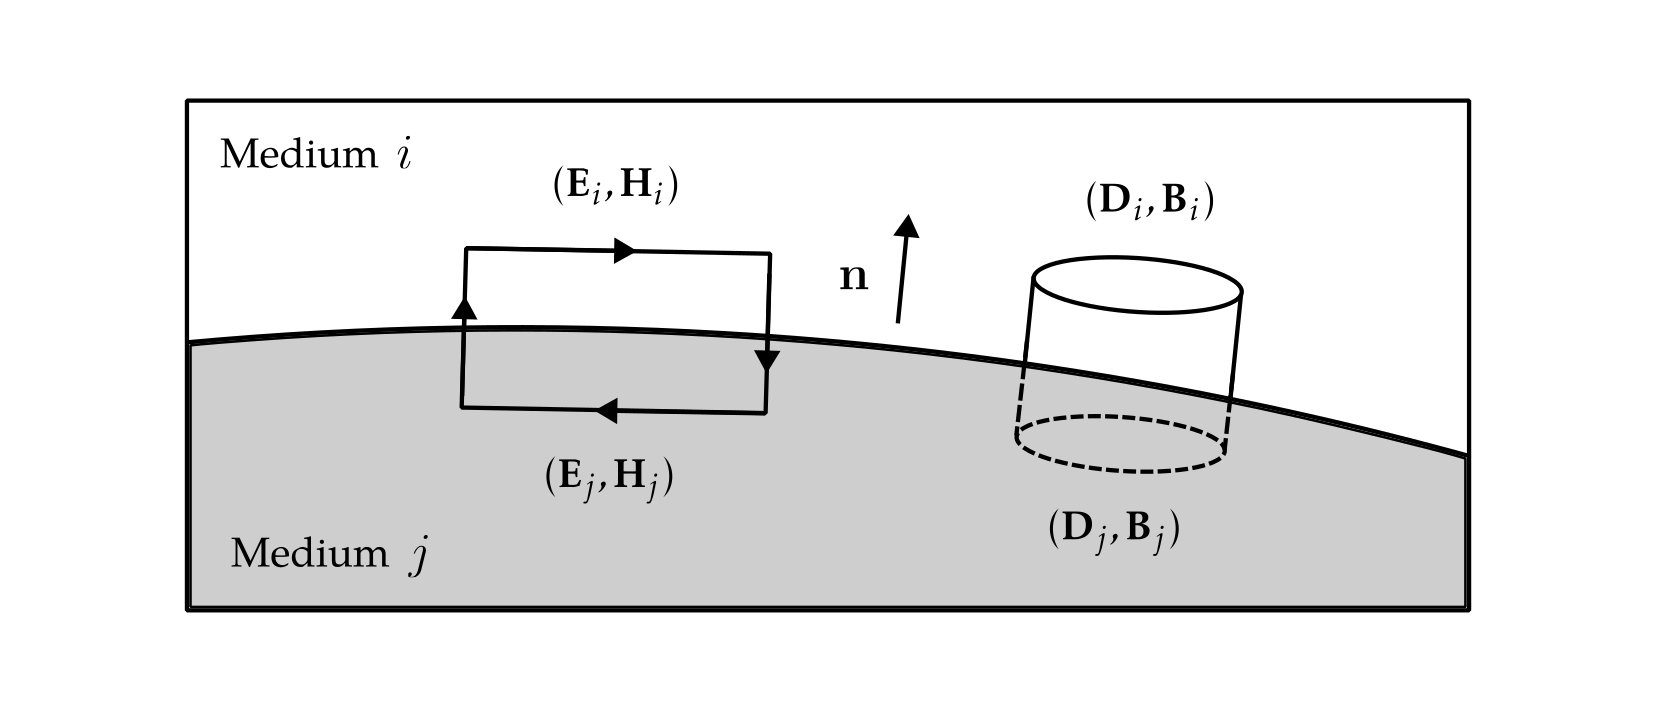
\includegraphics{figures/bcs.png}}%%
%        \caption{Boundary conditions between two material interfaces ($i,j$) in electromagnetic problems. Stoke's theorem gives the tangential field
%        conditions ($\mathbf{E}, \mathbf{H}$), while Gauss's theorem gives the normal field conditions ($\mathbf{D}, \mathbf{B}$).}
%        \label{fig:bcs}
%    \end{figure}

    \subsection*{Some useful properties of Maxwell's equations}
    The following are some key properties of Maxwell's equations that will be
    useful throughout this thesis:
    \begin{itemize}
        \item \textbf{Linearity and superposition:} The operator $\mathcal{L}$ in~\eqref{eq:maxwell_op} is linear, so any linear combination of solutions is
              also a solution, in accordance with the superposition principle.
              For example, given two solutions $\mathbf{E}_1$ and $\mathbf{E}_2$ to the
              linear systems $\mathcal{L}[\mathbf{E}_1] = \mathbf{f}_1$ and
              $\mathcal{L}[\mathbf{E}_2] = \mathbf{f}_2$,
              and two constants $\alpha$ and $\beta$, the combination $\mathbf{E}_3 =
                  \alpha \mathbf{E}_1 + \beta \mathbf{E}_2$ satisfies
              \begin{equation}
                  \mathcal{L}[\mathbf{E}_3] = \alpha \mathcal{L}[\mathbf{E}_1] + \beta
                  \mathcal{L}[\mathbf{E}_2] = \alpha \mathbf{f}_1 + \beta \mathbf{f}_2 =
                  \mathbf{f}_3\,.
              \end{equation}
              Hence, scaling the source term results in a proportionally scaled field
              solution. Note that this property is not valid when the source term or material
              properties depend on the field itself, making the operator nonlinear (e.g., \secref{sec:thermo_strong_coupling},
              \secref{sec:mech_strongly_coupled} and \secref{sec:laser}). In such
              cases the problem can be linearized for small nonlinearities
              using perturbation theory (\secref{sec:laser})~\cite{ownpub4}.

              \item \textbf{Hermiticity:} The operator $\mathcal{L}$ in~\eqref{eq:maxwell_op} is hermitian,
              meaning that the inner product of two solutions is invariant under the
              operator
                           %\begin{equation}
                           %    \int \mathbf{E}_1^* \cdot \mathcal{L}[\mathbf{E}_2] \d \mathbf{r} =
                           %    \int \mathcal{L}[\mathbf{E}_1]^* \cdot \mathbf{E}_2 \d \mathbf{r}\,,
                           %\end{equation}
                           \begin{equation}\label{eq:hermiticity}
                             \langle \mathbf{E}_1, \mathcal{L}[\mathbf{E}_2] \rangle = \langle \mathcal{L}[\mathbf{E}_1], \mathbf{E}_2 \rangle\,,
                         \end{equation}
              where in electromagnetic systems the inner product between two fields is conventionally defined as
                         \begin{equation}
                             \langle \mathbf{E}_1, \mathbf{E}_2 \rangle = \int_\Omega \mathbf{E}_1^*(\mathbf{r}) \cdot \mathbf{E}_2(\mathbf{r}) \, \d\Omega\,,
                         \end{equation}
              for an integration volume $\Omega$.
              The hermiticity property (\eqref{eq:hermiticity}) implies real eigenvalues and orthogonal eigenmodes\footnote{Except in
              the case of degeneracy, where orthogonality is not guaranteed.} in the generalized eigenvalue problem (\eqref{eq:gen_eigen}), as discussed
              in~\cite{phot_crys}.
              
              Although the operator $\mathcal{L}$ itself is an indefinite operator~\cite{phot_crys}, each of its constituent operators $\mathcal{L}_1[\square]=\nabla \times (\nabla \times \square)$ and $\mathcal{L}_2[\square]=\varepsilon_r(\mathbf{r}) \cdot \square$ are \textbf{positive semi-definite}, so all
              eigenvalues ($\omega_\lambda^2$) in the generalized eigenvalue problem (\eqref{eq:gen_eigen}) are nonnegative~\cite{phot_crys}. 
              
              However, for materials with
              gain or loss
              ($\varepsilon_r^{\prime\prime} \neq 0$ in~\eqref{eq:perm}) or some boundary conditions, the operators $\mathcal{L}$ and $\mathcal{L}_2$ become non-hermitian. In addition, the operator $\mathcal{L}_2$ becomes \textbf{indefinite} and eigenvalues can be positive, negative, or zero. For example, this occurs in lossy
              material systems
              (e.g., lossy metals in~\secref{sec:TOPS}~\cite{ownpub0}) and in lossy cavities~\cite{ownpub4},
              where the imaginary part of the mode frequency ($\Im\{\omega_\lambda\}$) is
              related to the modal decay rate, and quantifies the energy loss in the system (\secref{sec:TOPS})~\cite{ownpub0}.

            %\item \textbf{Scale-invariance:} The Maxwell operator $\mathcal{L}(\mathbf{r})$ is scale-invariant, which means that if $\mathbf{E}(\mathbf{r})$ solves Maxwell's equations at frequency $\omega$, then $\mathbf{E}(\alpha \mathbf{r})$ is a solution at $\omega' = \alpha \omega$, 
            %provided the dielectric function satisfies $\varepsilon(\omega, \mathbf{r}) = \varepsilon(\omega', \alpha \mathbf{r})$~\cite{phot_crys}. 
            %Thus, in systems where $\varepsilon$ is invariant under scaling, there is no fundamental length scale or permittivity value. However, since $\varepsilon(\omega) \neq \varepsilon(\omega')$ in general, this scale-invariance is typically broken. Nevertheless,
            %this property is interesting from the perspective of inverse design, where for a choice of permittivity when can design a device that can arbitrarily be scaled up or down in dimension.

        % \item \textbf{Conservation laws:} Maxwell's equations inherently satisfy
        %       several conservation laws, which are fundamental to physical systems MAKE SURE
        %       OF THE SYMBOLS AND EQUATIONS THEY ARE TIME-DOMAIN:
        %       \begin{itemize}
        %           \item \textbf{Charge conservation:} The continuity equation ensures
        %                 that charge is conserved in the system:
        %                 \begin{equation}
        %                     \nabla \cdot \bm{\mathcal{J}} + \frac{\partial
        %                         \mathcal{\rho}}{\partial t} = 0.
        %                 \end{equation}
        %                 This equation relates the divergence of the current density
        %                 $\mathbf`{J}$ to the time rate of change of the charge density $\mathcal{\rho}$.

        %           \item \textbf{Energy conservation:} The Poynting theorem describes the
        %                 conservation of electromagnetic energy:
        %                 \begin{equation}
        %                     \nabla \cdot \mathbf{S} + \frac{\partial \mathcal{U}}{\partial t} =
        %                     -\mathbf{J} \cdot \mathbf{E},
        %                 \end{equation}
        %                 where $\mathbf{S} = \mathbf{E} \times \mathbf{H}$ is the Poynting
        %                 vector representing the energy flux, and $\mathcal{U} = (1/2) (\varepsilon
        %                     |\mathbf{E}|^2 + \mu |\mathbf{H}|^2)$ is the electromagnetic energy density.

        %           \item \textbf{Momentum conservation:} The electromagnetic fields carry
        %                 momentum, and the conservation of momentum is described by the Maxwell stress
        %                 tensor $\mathbf{T}$:
        %                 \begin{equation}
        %                     \nabla \cdot \mathbf{T} + \frac{\partial \mathbf{p}}{\partial t} =
        %                     \mathbf{f},
        %                 \end{equation}
        %                 where $\mathbf{p}$ is the momentum density and $\mathbf{f}$ is the
        %                 force density acting on the system. The electromagnetic fields also carry
        %                 \textbf{angular momentum}, and its conservation is described by the angular
        %                 momentum density $\mathbf{L}$:
        %                 \begin{equation}
        %                     \frac{\partial \mathbf{L}}{\partial t} + \nabla \cdot
        %                     \mathbf{M} = \boldsymbol{\tau},
        %                 \end{equation}
        %                 where $\mathbf{M}$ is the angular momentum flux density
        %                 tensor, and $\boldsymbol{\tau} = \mathbf{r} \times \mathbf{f}$ represents the
        %                 torque density acting on the system.
        %       \end{itemize}

        %       TIE THIS TO PUBLICATION ENGINEERING

        \item \textbf{Time-reversal symmetry:} Maxwell's equations remain valid if
              we reverse the direction of time ($t\to-t$). It can be shown that under
              time-reversal symmetry
              the fields transform as
              $\bm{\mathcal{E}}(\mathbf{r}, t)\to\bm{\mathcal{E}}(\mathbf{r}, -t)$,
              $\bm{\mathcal{D}}(\mathbf{r}, t)\to\bm{\mathcal{D}}(\mathbf{r}, -t)$,
              $\bm{\mathcal{H}}(\mathbf{r},
                  t)\to-\bm{\mathcal{H}}(\mathbf{r}, -t)$, and $\bm{\mathcal{B}}(\mathbf{r},
                  t)\to-\bm{\mathcal{B}}(\mathbf{r}, -t)$, while the current density and charge
              density transform as
              $\bm{\mathcal{J}}(\mathbf{r},
                  t)\to-\bm{\mathcal{J}}(\mathbf{r}, -t)$ and $\varrho_q(\mathbf{r},
                  t)\to \varrho_q (\mathbf{r}, -t)$, respectively~\cite{reciprocity}.
              Applying these transformations
              to Maxwell's equations (\eqref{eq:faraday}--\eqref{eq:Gauss_B}) shows
              that the equations remain invariant under time reversal. 
              
              This
              symmetry can be extended by
              considering \textbf{parity-time (PT) symmetry}, which combines time-reversal
              with spatial inversion ($\mathbf{r}\to-\mathbf{r}$) and is satisfied for
              materials with refractive index $n(\mathbf{r}) = n^*(-\mathbf{r})$~\cite{pt}. There
              are however, some situations where time-reversal symmetry and/or PT symmetry is
              broken,
              such as in the presence of
              non-reciprocal materials (e.g., magneto-optical materials) or materials with
              optical losses (\secref{sec:TOPS}~\cite{ownpub0}).

              \item \textbf{Reciprocity:} In an optical system, the source and the
              detector of electromagnetic fields can be interchanged without changing the
              physical situation. For two volumes $\Omega_1$ and
                           $\Omega_2$
              with two current densities $\mathbf{j}_1$ and $\mathbf{j}_2$ that create
              the fields $\mathbf{E}_1$, $\mathbf{H}_1$ and $\mathbf{E}_2$, $\mathbf{H}_2$
              respectively, it is possible to show that via Lorentz reciprocity~\cite{novotny}
                           \begin{equation}\label{eq:reciprocity}
                               \int_{\Omega_1} \mathbf{j}_1 \cdot  \mathbf{E}_2 \d \Omega = \int_{\Omega_2}
                               \mathbf{j}_2 \cdot  \mathbf{E}_1 \d \Omega\,.
                           \end{equation}
              For lossless media ($\varepsilon_r^{\prime\prime} = 0$ in~\eqref{eq:perm}), this is equivalent to time-reversal symmetry, but for
              lossy systems, where time-reversal symmetry breaks down, reciprocity remains valid~\cite{Carminati:98}. Reciprocity
              is a very useful property of Maxwell's equations, as it can be used to
              greatly simplify some formulations of inverse design problems. For example, it has been used in device design for
              scintillation~\cite{Roques_Carmes_2022}, incoherent light emission~\cite{LED_opt, Yao_2022}, and nanolasers (\secref{sec:laser})~\cite{ownpub4}, among others.
    \end{itemize}

    %\subsection*{Point-like emitters: the Green's function formalism}

    %TODO: Add if we do coupled-emitter project.

    \section{The finite element method in electromagnetics}\label{sec:fem}
 The frequency-domain Maxwell wave equation introduced in \eqref{eq:wave_eq} can be solved numerically with \textbf{the finite element method}, as covered in detail 
 in many textbooks~\cite{jin, fem_book}. The main idea is to discretize the domain into a finite number of elements (e.g., tetrahedra, hexahedra), and then approximate the solution
 within each element using piecewise polynomial basis functions, also known as the shape functions. 
 
 In electromagnetic problems, vector-valued edge elements, known as Né\-dé\-lec elements~\cite{nedelec}, 
 are a natural choice. They are specifically designed to represent divergence-free fields and 
 to enforce the continuity of the tangential electric field across element boundaries, fullfulling the boundary condition in~\eqref{eq:BC_E}.
 The shape functions associated with Nédélec elements can be used to represent the electric field inside a finite element as
    \begin{equation}\label{eq:ned_shape}
 \boldsymbol{E}^e(\mathbf{r})=\sum^M_i \boldsymbol{N}_i(\mathbf{r}) E_i\,,
    \end{equation}
 where $M$ denotes the number of edges in the element, $\boldsymbol{N}_i$ denotes the shape functions, and $E_i$ is the value of the degrees-of-freedom of the electric field associated with each edge $i$. As an example
  of domain discretization, \figref{fig:fem} shows the two-dimensional domain introduced in \figref{fig:top_opt}, discretized
   into triangular first-order Nédélec elements~\cite{nedelec}. For illustration, the shape function corresponding to one of the edges is visualized.

    \begin{figure}[tb]
        \centering

        \makebox[\textwidth][c]{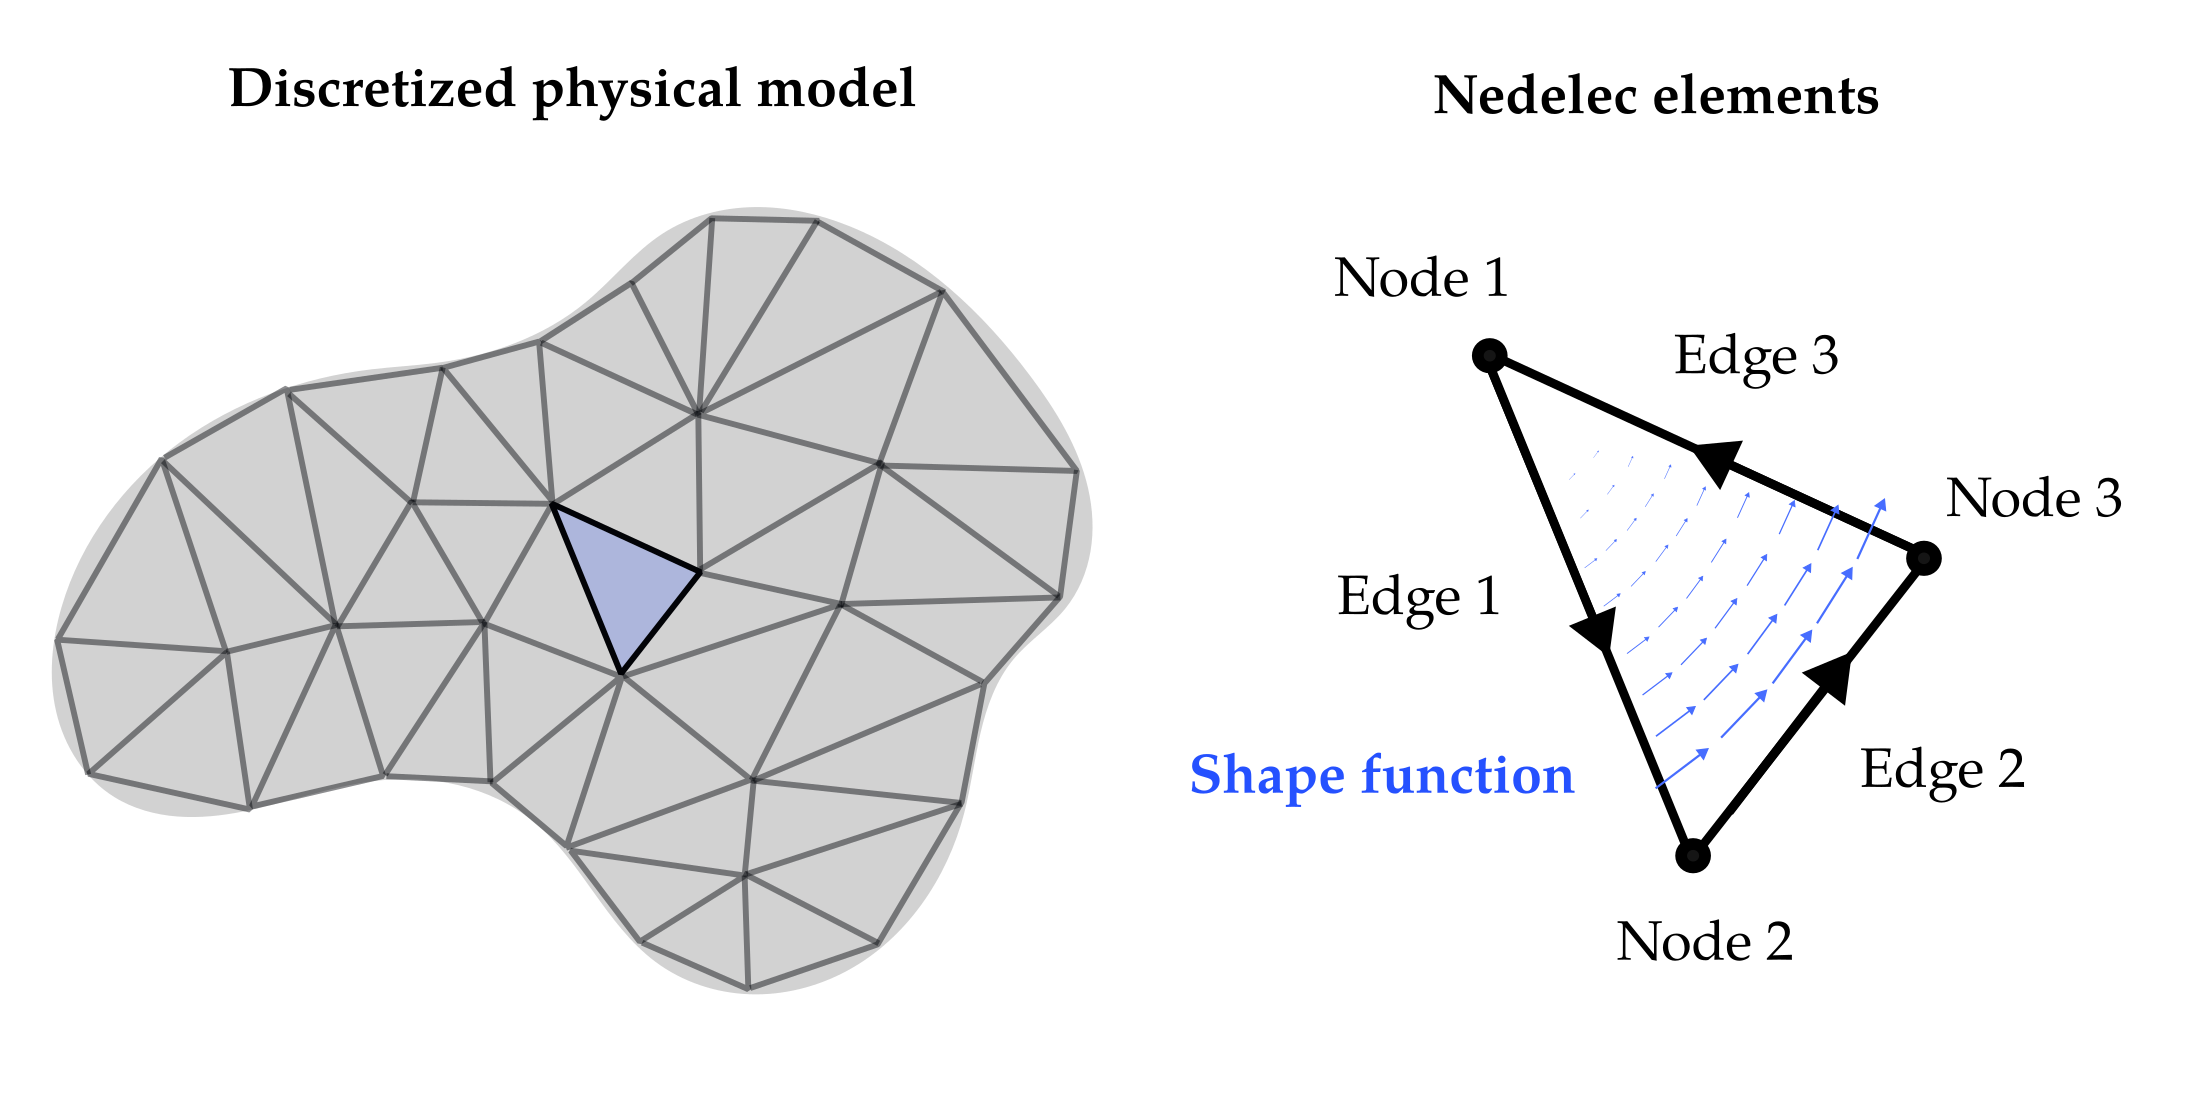
\includegraphics{figures/FEM.png}}%%
        \caption{Geometrical discretization of the physical domain into the finite-element mesh, which is composed of first-order Nédélec elements. The element colored
 in light blue is a triangular element with three edges, where
 we have sketched a quiver plot for the shape function for Edge
 2 $(\mathbf{N}_2)$.}
        \label{fig:fem}
    \end{figure}
    
 To derive the finite element formulation, the first step is to rewrite the governing partial differential equation in its weak (variational) form. This is done by multiplying the frequency-domain wave equation (\eqref{eq:wave_eq}) by a suitable test function, integrating over the computational domain, and applying integration by parts\footnote{Note that the weak form will be different for two-dimensional problems \cite{ownpub0, ownpub2}.}
    \begin{align}\label{eq:weak_form}
        \int_\Omega \left[ \left( \nabla \times \mathbf{v} \right) \cdot \left( \nabla \times \mathbf{E} \right)- \left(\frac{\omega}{c}\right)^2 \mathbf{v}\cdot(\varepsilon_r \mathbf{E})\right]& \d \Omega \nonumber \\ 
 - \int_{\Gamma} \mathbf{v} \cdot \left[ \mathbf{n} \times \left( \nabla \times \mathbf{E} \right) \right]& \d \Gamma 
 = \int_\Omega \mathbf{v} \cdot \mathbf{f} \d \Omega\,,
    \end{align}
 where $\mathbf{v}$ is the test function, $\Omega$ is the volume of the computational domain, and $\Gamma$ is the boundary where Neumann boundary conditions
 are prescribed. 
 
 By using
 the standard Galerkin method (where the test and basis functions are the same),
 one can discretize the weak form in \eqref{eq:weak_form} 
 into matrix form, yielding a linear system of equations
    \begin{equation}\label{eq:discretized}
 \mathbf{K} \mathbf{E} = \mathbf{F},
    \end{equation}
 which is solved for the vector $\mathbf{E}$ containing the degrees-of-freedom of the electric field, for a given stiffness matrix $\mathbf{K}$ that encodes the operator 
 in~\eqref{eq:maxwell_op}, and a 
 vector $\mathbf{F}$ containing the degrees of freedom of the forcing term. 
 As mentioned previosly\footnote{See discussion on hermiticity (\eqref{eq:hermiticity})
 in~\secref{sec:nanophotonics}.} the stiffness matrix is a sparse symmetric indefinite matrix,
 restricting the use of iterative solvers
 (e.g., Cholesky factorization, the Krylov method) to solve the system of equations.
 Thus, LU factorization (via sparse direct solvers) is
 a common choice for topology optimization applications, since one can reuse the factorization to solve
 the adjoint problem (e.g., \eqref{eq:adjoint_eqs} in~\secref{sec:topopt_theory}). 
 
 To reduce the computational cost of solving the system of equations in (\eqref{eq:discretized}), symmetry conditions can be applied by employing perfect electric conductor ($\mathbf{n} \times \mathbf{E}=0$) and perfect
 magnetic
 conductor ($\mathbf{n} \cdot \mathbf{H}=0$) boundary conditions at the symmetry-plane boundaries.

 \section{Beyond single-physics -- coupled photonic systems}\label{sec:coupled}

 Coupled multiphysics systems are physical systems where the solution to one physical 
 problem depends on the solution of another. For example, in the coupled multiphysics 
 problem studied in~\cite{ownpub0}, the optical field depends on the temperature profile via
 the temperature-dependent refractive index. Thus, one first needs to solve a heat transfer problem [e.g., via the finite element method (\secref{sec:fem})] to find the temperature distribution. 
 This temperature distribution is then used to calculate the refractive index, which is needed to solve the optical problem.
    \subsection*{Two linearly coupled problems}
 Let us consider a more general scenario than the previous example, where two physical
 problems can be described by linear partial differential equations. Following the notation in~\eqref{eq:maxwell_op}, the
 first problem
 is described by the equation $\mathcal{L}_1 [\mathbf{u}_1]= \mathbf{f}_1$ and
 the second problem is described by the
 equation $\mathcal{L}_2 [\mathbf{u}_2]= \mathbf{f}_2$, where $\mathbf{u}_1$ and $\mathbf{u}_2$ denote the solutions to the linear problems. Using the finite element method (\secref{sec:fem}), these equations can be
 discretized into the form $\mathbf{K}_1 \mathbf{u}_1 = \mathbf{f}_1$ and $\mathbf{K}_2 \mathbf{u}_2 =
\mathbf{f}_2$.
 If the stiffness matrix ($\mathbf{K}_1$, $\mathbf{K}_2$) and/or loading term ($\mathbf{f}_1$, $\mathbf{f}_2$) of one of the problems depends on the solution of the
 other problem, we say that the two physics problems are
    \textbf{coupled}. 
    
    For \textbf{linearly coupled problems}, it is possible to write out the two equations as a system of equations
    \begin{equation}\label{eq:c_N_2}
 \mathbf{K} \mathbf{u} = \mathbf{f} \quad \longleftrightarrow \quad 
        \begin{bmatrix}
 \mathbf{K}_1  & \mathbf{C}_{12} \\
 \mathbf{C}_{21} & \mathbf{K}_2
        \end{bmatrix}
        \begin{bmatrix}
 \mathbf{u}_1 \\
 \mathbf{u}_2
        \end{bmatrix}
 =
        \begin{bmatrix}
 \mathbf{f}_1^\prime \\
 \mathbf{f}_2^\prime
        \end{bmatrix}\,,
    \end{equation}
 where $\mathbf{C}_{12}$ is the linear term that couples physics $2$ to physics $1$,
$\mathbf{C}_{21}$ is the linear term that couples physics $1$ to physics $2$, and the
 prime ($\prime$) denotes that we have rewritten the loading terms so that they do not
 depend on the solution vector, ensuring that all couplings are
 accounted for in the coupling terms. 
 
 If the coupling
 matrices in~\eqref{eq:c_N_2} are non-zero ($\mathbf{C}_{12}\neq 0$ and $\mathbf{C}_{21}\neq 0$), we
 say that physics $1$ and $2$ are
    \textbf{strongly coupled}, since there is feedback between the two physics. If the
 coupling matrices are zero $\mathbf{C}_{12}=\mathbf{C}_{21}=0$, we say that the
 physics
 are \textbf{decoupled}, since they can be solved independently. Lastly, in the
 case where $\mathbf{C}_{12}\neq 0$ ($\mathbf{C}_{21}\neq 0$) but $\mathbf{C}_{21} = 0$ ($\mathbf{C}_{12} = 0$) we say that the
 physics are \textbf{weakly
 coupled} since the solution of physics $1$ ($2$) depends on the solution of physics
$2$ ($1$), but not vice versa.

\subsection*{$N$ linearly coupled problems}

 In the case of $N$ coupled problems, the system of equations in the $N=2$ case (\eqref{eq:c_N_2}) generalizes to
    \begin{equation} \label{eq:multiphysics_strong}
        \begin{bmatrix}
 \mathbf{K}_1    & \mathbf{C}_{12} & \cdots & \mathbf{C}_{1N} \\
 \mathbf{C}_{21} & \mathbf{K}_2    & \cdots & \mathbf{C}_{2N} \\
            \vdots          & \vdots          & \ddots & \vdots          \\
 \mathbf{C}_{N1} & \mathbf{C}_{N2} & \cdots & \mathbf{K}_N
        \end{bmatrix}
        \begin{bmatrix}
 \mathbf{u}_1 \\
 \mathbf{u}_2 \\
            \vdots       \\
 \mathbf{u}_N
        \end{bmatrix}
 =
        \begin{bmatrix}
 \mathbf{f}_1 \\
 \mathbf{f}_2 \\
            \vdots       \\
 \mathbf{f}_N
        \end{bmatrix}\,,
    \end{equation}
 where we have dropped the prime notation for convenience. Following a similar logic as in the $N=2$ case (\eqref{eq:c_N_2}), if
 the coupled
 system is defined by an upper or lower triangular matrix, we can say that the
 system is weakly coupled. 
    %For matrices with more non-diagonal
    %zero entries the system will be strongly coupled, while if there are more
    %non-diagonal zero entries than non-zero entries, we can say that the system is
    %weakly coupled. 
 Similarly, for a diagonal matrix, the system will be decoupled, and the equations can be
 solved independently.

 \subsection*{Weak nonlinear coupling}


In this thesis, we consider the case of \textbf{weak nonlinear coupling},
 which is common in many
 coupled multiphysics problems. As an example of a system with weak nonlinear coupling, we consider the problem discussed in \secref{sec:TOPS}~\cite{ownpub0}, where the refractive index encoded in 
 the stiffness matrix depends on the solution of the temperature field.
 In this scenario, the system of equations is based on an upper (or lower) triangular matrix, where the stiffness matrices and the coupling matrices for a given physics may depend 
 on the solutions of subsequent problems in a cascaded fashion, yielding the system
     \begin{equation} \label{eq:multiphysics_weak_nonlinear}
        \begin{bmatrix}
 \mathbf{K}_1(\mathbf{u}_2, \cdots \mathbf{u}_N)    & \mathbf{C}_{12} (\mathbf{u}_2, \cdots \mathbf{u}_N)& \cdots & \mathbf{C}_{1N}(\mathbf{u}_2, \cdots \mathbf{u}_N) \\
            \mathbf{0} & \mathbf{K}_2 (\mathbf{u}_3, \cdots \mathbf{u}_N)   & \cdots & \mathbf{C}_{2N} (\mathbf{u}_3, \cdots \mathbf{u}_N)\\
            \vdots          & \vdots          & \ddots & \vdots          \\
            \mathbf{0} & \mathbf{0} & \cdots & \mathbf{K}_N
        \end{bmatrix}
        \begin{bmatrix}
 \mathbf{u}_1 \\
 \mathbf{u}_2 \\
            \vdots       \\
 \mathbf{u}_N
        \end{bmatrix}
 =
        \begin{bmatrix}
 \mathbf{f}_1\\
 \mathbf{f}_2\\
            \vdots       \\
 \mathbf{f}_N
        \end{bmatrix}\,,
    \end{equation}
 where we have chosen the upper triangular form of the matrix.
 Note that when there are non-zero entries in the lower triangle of the matrix, or the stiffness or coupling matrix of a given problem depends on the solution to a previous problem, the system of equations is strongly coupled and fully nonlinear.

 \subsection*{Solving the coupled system of equations}

 In general, there are two main strategies for solving coupled problems. For strongly coupled problems, 
 such as the one presented in~\eqref{eq:multiphysics_strong}, a \textbf{monolithic} approach is often used, in which the entire system of 
 equations is solved simultaneously, for example, using direct solvers like LU factorization. When this is not feasible or 
 efficient, a \textbf{segregated} approach may be used instead, solving the coupled problems in an iterative sequence. In this 
 approach, each subproblem is addressed separately, with the solution of one problem used to update the others. This process 
 is repeated until a convergence criterion is met (e.g., \secref{sec:mech_strongly_coupled}~\cite{ownpub5}). In weakly coupled systems, the solution of one subproblem feeds directly into the next. 
 As a result, each problem only needs to be solved once to obtain the full solution. This is also the case for 
 weak nonlinear coupling (\eqref{eq:multiphysics_weak_nonlinear}), where even if the coupling is nonlinear, the system of equations
 can be solved by solving $N$ seggregated linear problems (e.g.,~\cite{ownpub0}).
    
 \section{Topology optimization framework}\label{sec:topopt_theory}
 Topology optimization (\secref{fig:top_opt})~\cite{topopt_book} can be used as a systematic design tool to optimize designs in numerically discretized multiphysics problems. 
 As an example, in \figref{fig:top_opt_multi}, we build on the depiction of the nanophotonic topology optimization problem presented in \figref{fig:top_opt}, by considering
 multiphysics effects, such as heat sources and mechanical forces.

 Seminal work by Sigmund~\cite{MEMS_multi} laid the foundation for \textbf{multiphysics topology optimization}, with the optimization of micro-electro-mechanical system (MEMS) devices. 
 Still today, multiphysics topology optimization is an active topic of research, where state-of-the-art multiphysics topology optimization is used to tackle complex coupled design problems; for instance, optimizing for thermo-mechanical~\cite{third_thermal}, magneto-mechanical~\cite{magneto}, or fluid-structure interaction~\cite{fsint} problems. 
 This has enabled highly efficient and integrated designs across engineering disciplines, but remains mainly uncharted territory for nanophotonic device optimization. In the remainder of this section, we will review the theory behind multiphysics topology optimization. For a more detailed overview of some problems in coupled multiphysics
 topology optimization, we refer the reader to the book chapter by Maute~\cite{coupled_topopt}.
    
    \subsection*{Optimization problem formulation}
    In multiphysics topology optimization, we consider a general constrained optimization problem 
    expressed as
    \begin{equation}
        \begin{array}{clr}
            \max\limits_{\rho}                        & \Psi(\rho, \mathbf{u}) \quad \quad \quad \quad \,\,\,\, 
              & \text { (Objective function) }                                                         \\
            \text { s.t. }                            & \mathbf{K}(\rho, \mathbf{u})\mathbf{u} -\mathbf{f} (\rho, \mathbf{u})=0 \quad
                     & \text { (State equations) }                                                            \\
                                                      & c_j(\rho, \mathbf{u}) \leq 0 \quad \quad \quad \quad \quad  \,\,\, \forall j \in\left[1,
            N_c\right]                                & \text { (Inequality constraints) }                                                     \\
                                                      & \rho_{\text {min }} \leq \rho \leq \rho_{\text {max }}                  & \text { (Box
                constraints) }
        \end{array}
    \end{equation}
    where the FOM ($\Psi$) is maximized for a design field $\rho$ with upper
    bound $\rho_{\text {max }}$ and lower bound $\rho_{\text {min }}$,
    subject to the residual of the state equation of the coupled multiphyiscs problem, and
     $N_c$ inequality constraints. The optimization problem is solved using
    the gradient-based algorithm of the Method of Moving
    Asymptotes (MMA)~\cite{MMA} or the Globally Convergent Method of Moving Asymptotes
    (GCMMA)~\cite{GCMMA}, by iteratively updating the design field until a
    termination criterion (e.g., maximum number of iterations) is met.

    \begin{figure}[bt]
      \centering
      \makebox[\textwidth][c]{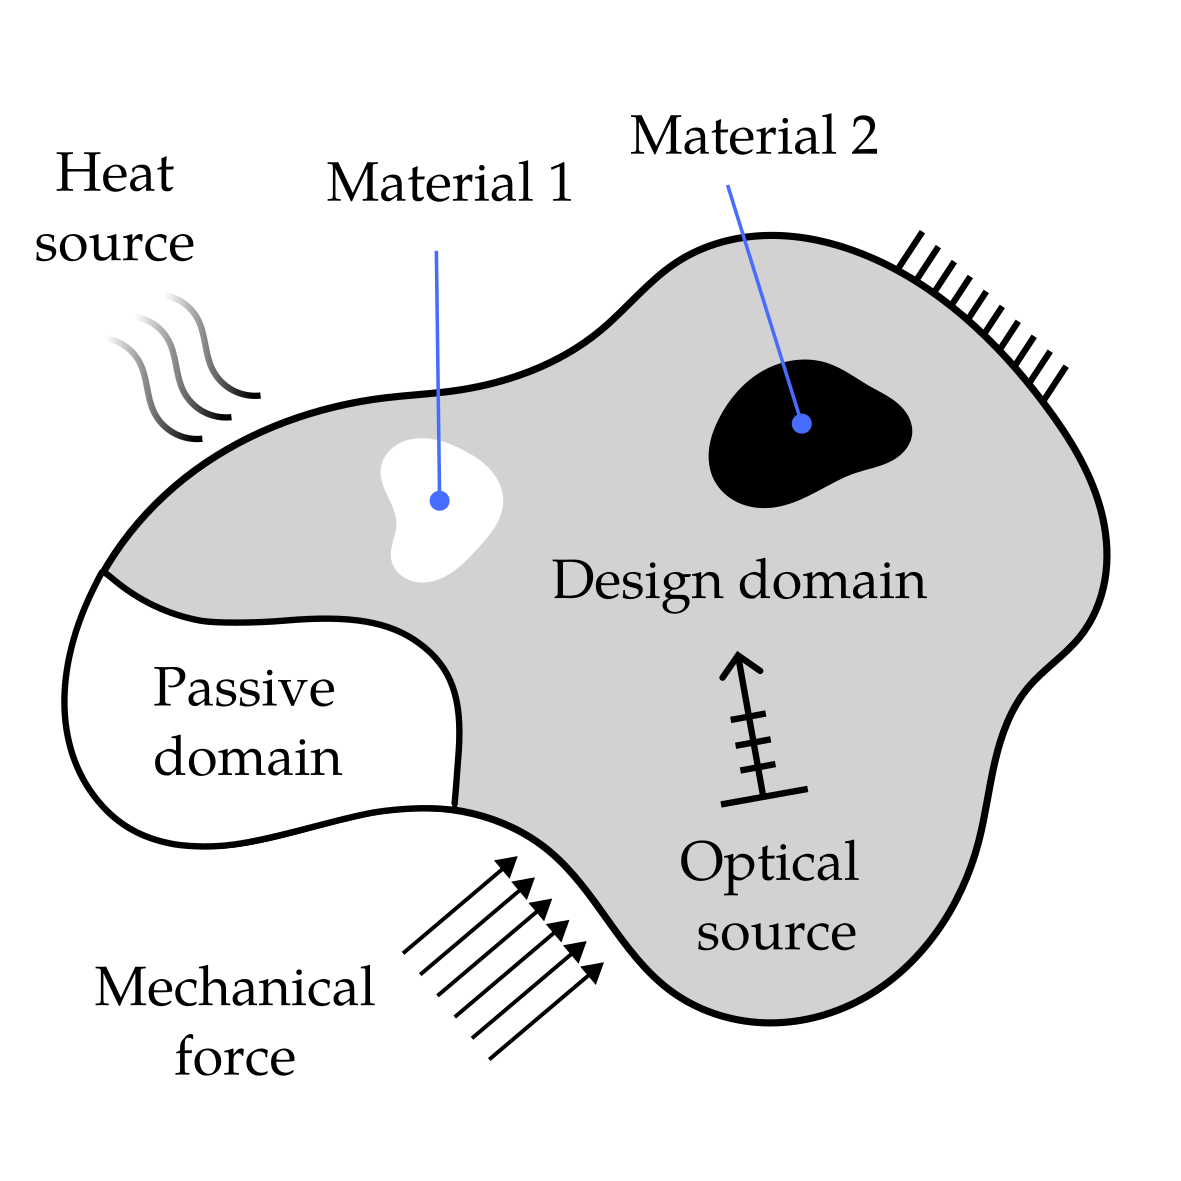
\includegraphics{figures/top_opt_multi.png}}%%
      \caption{Topology optimization of a multiphysics system, which accounts for thermal, mechanical, and optical effects. The system is excited by a thermal source, a mechanical force, and an optical source. The simulation domain comprises a passive domain (white) where the material is fixed, and a design domain (grey), where the material distribution is optimized for two different materials.}
          \label{fig:top_opt_multi}
   \end{figure}

    \subsection*{From densities to material properties}
    To regularize the optimization and introduce a weak sense of geometric length
    scale, we filter
    the design field using a \textbf{filter operation}. The filtered design field can
    be calculated using a
    convolution-based filter operation~\cite{projection}
       \begin{equation}\label{eq:filter_conv}
           \begin{aligned}
                & \tilde{\rho}(\mathbf{r})=\frac{\sum_{k \in \mathcal{B}_{e, h}}
    w\left(\mathbf{r}-\mathbf{r}_k\right) A_k \rho_k}{\sum_{k \in \mathcal{B}_{e,
    h}} w\left(\mathbf{r}-\mathbf{r}_k\right) A_k}\,,                              \\
                & w(\mathbf{r})=\left\{r_f-|\mathbf{r}| \quad \forall|\mathbf{r}| \leq r_f,
    \quad r_f \geq 0\right.\,,
           \end{aligned}
       \end{equation}
   
    where $A_k$ is the area of the $k^\text{th}$ element, and $\mathcal{B}_{e, h}$ denotes
    the
   $h^\text{th}$ set of finite elements whose center point is within a filter
    radius $r_f$ of the
   $h^\text{th}$ element. One can also filter by solving a Helmholtz-type
    PDE~\cite{PDE_filter}
       \begin{equation}
    -\left(\frac{r_f}{2 \sqrt{3}}\right)^2 \nabla^2
    \tilde{\rho}+\tilde{\rho}=\rho\,.
       \end{equation}
    The filter operation is followed by a \textbf{smoothed Heaviside
    threshold}~\cite{projection}
       \begin{equation}\label{eq:threshold}
    \hat{\rho} \equiv \Theta_{\beta,\eta}(\tilde{\rho}) =\frac{\tanh (\beta \cdot \eta)+\tanh \left[ \beta
               \cdot(\tilde{\rho}-\eta) \right]}{\tanh (\beta \cdot \eta)+\tanh \left[ \beta \cdot(1-\eta) \right]}\,,
    \quad \beta \in[1, \infty)\,,\, \eta \in[0,1]\,,
       \end{equation}
    to obtain the physical field $\hat{\rho}$, where $\beta$ and $\eta$ control the threshold sharpness and value in the 
    threshold function $\Theta_{\beta,\eta}(\tilde{\rho})$,
    respectively. Note that in topology optimization problems the threshold sharpness ($\beta$) is gradually increased as the optimization progresses, which is also known as 
    the continuation scheme. This ensures that
    small $\beta$ allows grayscale designs in which the topology can change smoothly, while larger
       $\beta$ binarize the structure, thus yielding physically realizable devices.
       
    As an example of filtering and thresholding, in 
       \figref{fig:ft} we consider a discretized circle design.
    The design field is filtered using the convolution filter (\eqref{eq:filter_conv}), with a radius of $r_f=4$ pixels, which smooths the field, removing sharp and localized
    geometrical features. Subsequently, the smoothed Heaviside threshold (\eqref{eq:threshold}) is applied with $\beta=100$ and $\eta=0.5$ to obtain the physical field. This field is projected towards binary 
    values, effectively removing all the values below $\eta$ and setting the rest to be solid ($\hat{\rho}=1$).
   
    \begin{figure}[tb]
        \centering

        \makebox[\textwidth][c]{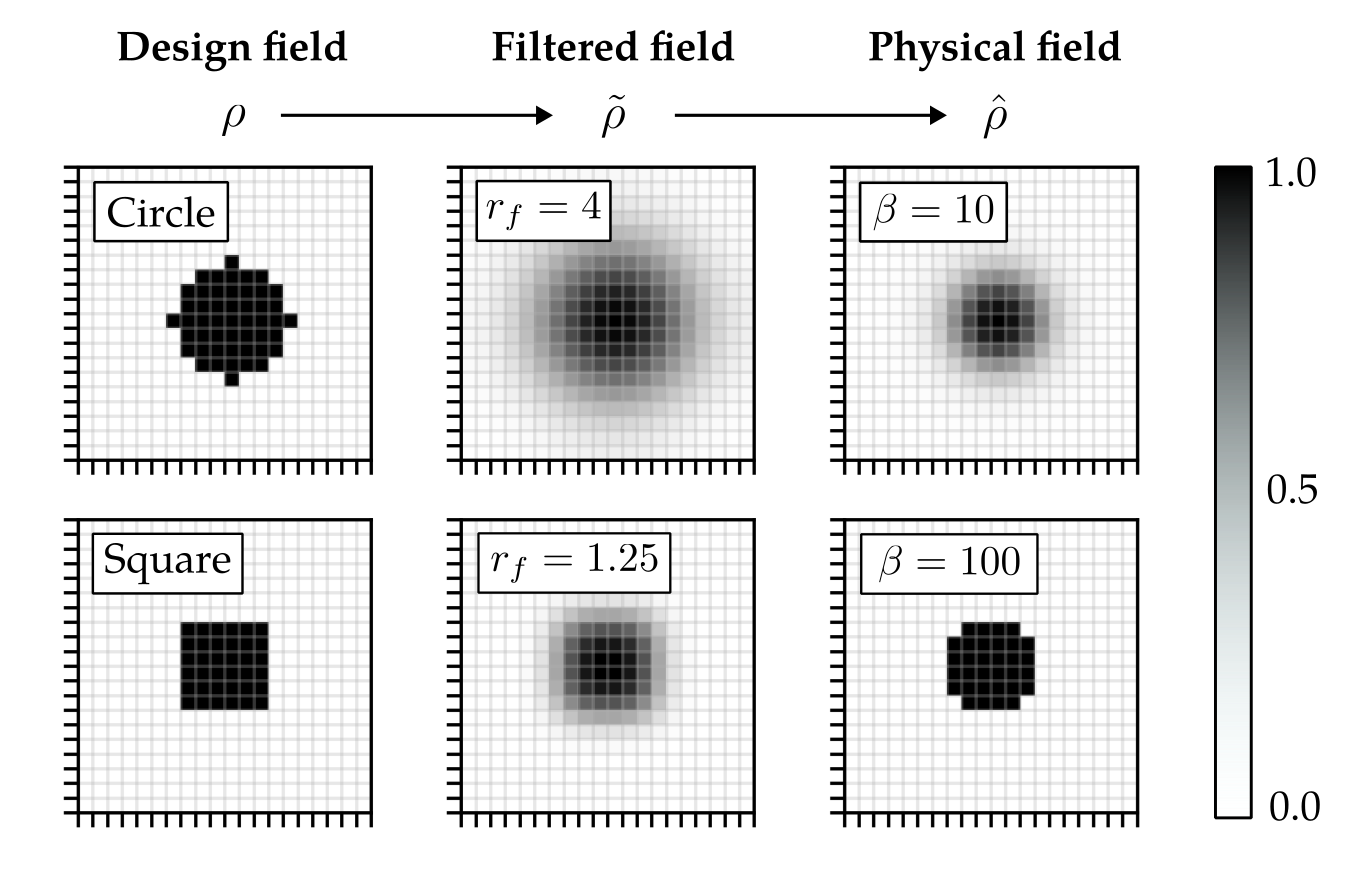
\includegraphics{figures/filter_threshold.png}}%%
        \caption{Effects of filtering and thresholding on the design field for the discretized
        version of a circle. In this example the filtering radius is $r_f=4$ pixels, the threshold sharpness is 
        $\beta=100$, and the threshold value is $\eta=0.5$.}
        \label{fig:ft}
    \end{figure}

    The physical field ($\hat{\rho}$) can be interpolated to the physical material properties (e.g., refractive index, Young's
    modulus) using a
    \textbf{material interpolation}. For example, the well-known Simplified Isotropic Material with Penalization (SIMP) material interpolation~\cite{SIMP} can be used
    \begin{equation}\label{eq:SIMP}
        \zeta(\hat{\rho})=\zeta_0+\hat{\rho}^p\left(\zeta_1-\zeta_0\right)\,,
    \end{equation}
 where $\zeta$ is the material property, $\zeta_0$ and $\zeta_1$ are the
 material properties of the void ($\hat{\rho}=0$) and solid ($\hat{\rho}=1$), respectively, and $p$
 is a penalization factor\footnote{Usually, $p=3$ for compliance optimization problems and $p$=1
 for other problems where a linear interpolation suffices (e.g.,~\cite{ownpub3,ownpub4}).}. Note that in some
 special cases, like topology optimization in optical problems with metals, it is beneficial
 to employ a non-linear material interpolation~\cite{nonlinear_interp,ownpub0} for the complex refractive index ($\underbar{n}=\zeta$, \eqref{eq:perm}).

    \subsection*{Adjoint sensitivity analysis}

    Adjoint sensitivity analysis provides an efficient way to calculate the gradient of the FOM with respect to the design variables,
 enabling gradient-based optimization. In this thesis, it is applied to multiphysics problems,
 where we consider the case of weakly coupled problems with
 nonlinear coupling (\eqref{eq:multiphysics_weak_nonlinear}) solved using a segregated approach, with the detailed derivations in 
    \appref{app:appendix1}. Note that for coupled problems solved with a monolithic approach, where all physics are handled
 in a single solve, the adjoint sensitivities can be computed directly by solving a single adjoint problem for the entire
 system (as shown in~\cite{jensen_review} for optical cases), with no additional derivations required.

 Following the derivations in \appref{app:appendix1}, the sensitivities for a weakly coupled problem with nonlinear coupling solved using the segregated
 approach can be computed as
    \begin{equation}
 \frac{\d \Psi}{\d \hat{\rho}}  = \frac{\partial \Psi}{\partial \hat{\rho}} + \sum^N_{i=1} \Lambda_{i}^{\top} \left( \frac{\partial \mathbf{K}_i}{\partial \hat{\rho}} \mathbf{u}_i - \frac{\partial \mathbf{f}_i}{\partial \hat{\rho}} + \sum^N_{j=i+1} \frac{\partial \mathbf{C}_{ij}}{\partial \hat{\rho}} \mathbf{u}_j \right)\,,
    \end{equation}
 where $N$ is the number of coupled problems and the Lagrange multipliers $\Lambda_i$ are the solution to the adjoint equations
    \begin{equation}\label{eq:adjoint_eqs}
      \mathbf{K}^\top_i \Lambda_i = -\left(\frac{\partial \Psi}{\partial \mathbf{u}_i}\right)^\top - \sum_{j=1}^{i-1} \left[ 
         \mathbf{u}^\top_j \left(\frac{\partial \mathbf{K}_j}{\partial \mathbf{u}_i}\right)^\top + \mathbf{C}^\top_{ji} + \sum^N_{k=j+1} \mathbf{u}^\top_k \left(\frac{\partial \mathbf{C}_{jk}}{\partial \mathbf{u}_i}\right)^\top \right]\Lambda_j  \quad \forall i \in [1, N] \,.
   \end{equation}
 Following these adjoint systems, one needs to solve the first adjoint equation ($i=1$) 
 and feed the solution to the following adjoint equation ($i=2$), and so on, until one can solve the last adjoint problem $i=N$; backwards compared to the forward problem (\eqref{eq:multiphysics_weak_nonlinear}).
 Note that by using this derivation, we can recover the sensitivities derived in~\cite{ownpub0} for a thermo-optical coupled problem ($N=2$), with weak nonlinear coupling
 via the stiffness matrix of the optical problem [$\mathbf{K}_1(\mathbf{u}_2)$ and $\mathbf{C}_{12}=\mathbf{C}_{21}=0$, where ``$1$'' refers to the optical problem and ``$2$'' refers to the 
 heat transfer problem].
    
 To recover the final sensitivities, one applies the chain rule with respect to the filtering and thresholding operations
    \begin{equation}
 \frac{\d \Psi}{\d \rho} = \frac{\partial \Psi}{\partial \hat{\rho}} \cdot \frac{\partial \hat{\rho}}{\partial \tilde{\rho}} \cdot \frac{\partial \tilde{\rho}}{\partial \rho}\,,
    \end{equation}
 where the final sensitivities $\d \Psi/\d \rho$ are the sensitivities used by the optimization algorithm.

%\section{A practical note on computational implementation}

%Using first order edge, or nodal, elements a rule of thumb is to include at
%least 10 elements per wavelength.

%Discuss direct vs iterative solvers, discuss condition number of the system.
%Sparsity, symmetry, definitiness
%Discuss the practical implementation, with COMSOL and other means (Fenics,
%gridap, etc).
%Check Niels, Ian's thesis, and other references.
%Bla bla bla...